% use paper, or submit
% use 11 pt (preferred), 12 pt, or 10 pt only

\documentclass[letterpaper, paper,11pt]{./AAS}		% for final proceedings (20-page limit)

\usepackage{bm}
\usepackage{amsmath}
\usepackage{subfigure}
\usepackage[colorlinks=true, pdfstartview=FitV, linkcolor=black, citecolor= black, urlcolor= black]{hyperref}
\usepackage{xfrac}
\usepackage{booktabs}

\begin{document}

\subsection{$\Delta V$EGA Maneuver Implementation}
A $\Delta V$EGA orbit, also referred to as a leveraging orbit specifically of Earth, launches with the intent to gravity assist off the body for a higher post-flyby heliocentric energy\cite{Hollenbeck}.  Leveraging orbits are classified by their nominal resonance period multiple with respect to the flyby body's heliocentric orbit, and we will refer to this number as "$k$." For example, a leveraging orbit that has a period roughly 3 times as large as Earth's will have a $k=3$ which is represented as a 3:1 $\Delta V$EGA trajectory. The actual period of these orbits will vary either greater than or less than the nominal time due to flying by the body at a different Earth heliocentric true anomaly. Trajectories with a larger period are referred to as $k$:$1^{+} \Delta$VEGA and those with a shorter are $k$:$1^{-} \Delta$VEGA trajectories. To modify the flyby Earth true anomaly a maneuver at the aphelion (deep space maneuver) is executed.


The deep space maneuver (DSM) and subsequent Earth launch characteristics are calculated before the tree generation in order to reduce the required number of computations within the search. We approximate the $\Delta V$ requirements for both maneuvers, and their inclusion reduces the discontinuous trajectory endpoint velocities needed to patch Earth-Earth flyby sequences. Having the required aphelion $\Delta V$ can also aid the optimization process initial guess. A lookup table sorted by the nominal resonance multiple ($k$) and encounter true anomalies ($\theta_{E}$) contains the resulting leveraging orbit properties and maneuver magnitudes. Due to being a rough approximation, the circular Earth orbit and coplanar trajectories assumptions are used. Finding the $\Delta V$EGA orbit parameters for a specific encounter true anomaly ($\theta_{E}$) and $k$ begins by assuming a nominal orbit period launch and its associated $V_\infty$. The state elements are computed at Earth and the resulting aphelion radius and velocity are found. Because the intercept true anomaly is fixed, its location and the time it takes to reach the point are known. Eq.~\eqref{eq:dteqn} is the difference in time from the DSM maneuver location to the Earth gravity assist (EGA) point where $\tau_E$ is the orbital period of Earth.
%
\begin{equation}
	\label{eq:dteqn}
	dt = k\tau_E \pm \tau_E(\theta_E/2\pi)
\end{equation}
%
%
\begin{figure}[htb]
	\centering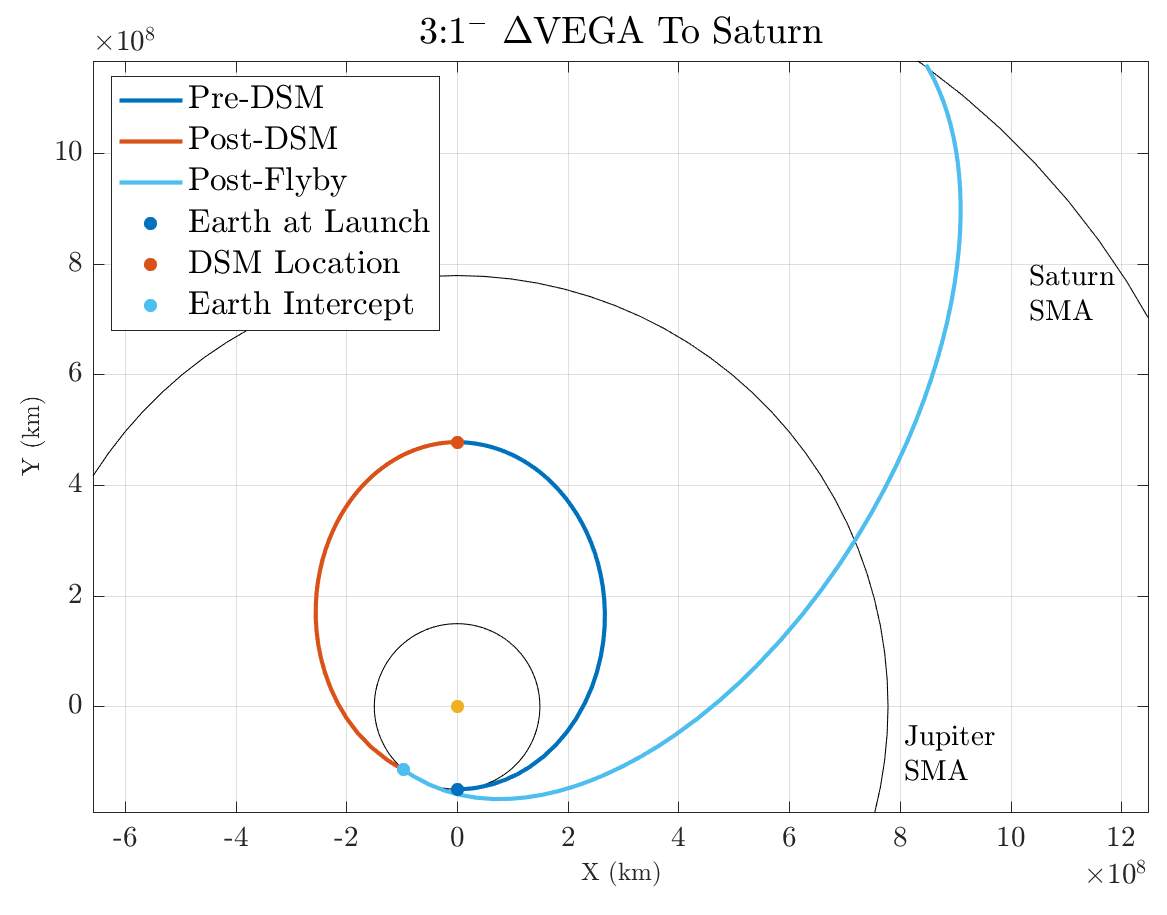
\includegraphics[width=3.6in]{./Figures/dsmmatlab}
	\caption{Example of a computed 3:$1^{-} \Delta$VEGA trajectory with a final aphelion radius roughly that of Saturn's semi-major axis. The launch $V_\infty$ is 6.97 km/s and the required DSM $\Delta V$ is 0.39 km/s. The EGA flyby altitude was constrained to 200 km, which yielded the highest post flyby energy.}
	\label{fig:dsmmatlab}
\end{figure}
%
\\A Lambert arc is computed between these points and the resulting initial velocity change is used to find the DSM vector. The final velocity vector is assumed to be the heliocentric velocity of the leveraging orbit at the EGA. The relative velocity, $\vec{\textbf{V}}_{\infty}$ is computed and a planar flyby of Earth can now be calculated from the tree search algorithm. Figure~\ref{fig:dsmmatlab} illustrates an example leveraging orbit being calculated for $\theta_{E}$ = 40.$7^{\circ}$. An energy maximizing flyby and propagation to the new aphelion is added to the end of the $\Delta V$EGA orbit to show the resulting trajectory.


From testing, we noticed that as $\mid\theta_E\mid$ increased, a normal component of the DSM $\Delta V$ appeared and grew larger. To limit the $\Delta V$ to only a tangential component, and in return to reduce the total $\Delta V$ required, a minimizer can be employed. This optimization comes at the expense of a higher launch energy and a longer flight time for trajectories requiring large $\mid\theta_E\mid$. Differing trends from Sims et. al. analysis of $V_\infty$ leveraging\cite{sims1994} were only noticed in high total $\Delta V$ cases for each $k$ leveraging orbit family. These solutions were discarded from the lookup table due to delivering lower aphelion radii post-flyby when compared to lower total $\Delta V$ leveraging orbits of the same family. The case presented in Figure~\ref{fig:dsmmatlab} is intended to matche that discussed by Sims et. al\cite{Sims1997} and has nearly identical results. The inclusion of deep space maneuvers, not specific to $\Delta V$EGAs, are not implemented in the current form of the tree search. However, because the algorithm patches the two conics forming the leveraging orbit using the Lambert's method, the possibility to extend DSM maneuvers for off-tangent $V_\infty$ departures and targeting for the flyby can be implemented. This inclusion adds another dimension to the lookup table but offers leveraging maneuvers between Earth and Venus.


Now that the $\Delta V$EGA orbit properties are known, the lookup table solution can be extended to the actual solar system model in the tree search. The table values are represented in a relative frame with respect to Earth's state vector at the launch epoch. A subsequent transformation of the departure velocity and pre-EGA incoming $\vec{\textbf{V}}_{\infty}$ can be done in order to find their specific components corresponding to an Earth epoch in the Ecliptic J2000 frame. From the initial node in the tree, a set of Earth leveraging time-of-flight nodes are created corresponding to their respective $k$ and $\theta_E$ parameters. The number of these leveraging nodes included in the initial flight time layer of the tree is directly related to the angular spacing of $\theta_E$. As the resolution becomes finer, by increasing the $\textit{detail}$ input, $d$, to the search, the estimated $\Delta V$ becomes more accurate. This, however, increases of the number of tree nodes created, and so for a rough idea of the trajectory search space, a coarse resolution is preferred. The discontinuous $\Delta V$ post-EGA required to patch the incoming leg from the leveraging orbit and outgoing leg to the next planet node will determine if the leveraging node and its performance is effective for the transfer. Using this method, a distinction between the $\Delta V$EGA trajectory families to different outer planets can be observed.


% Force the text below to next page
\phantom{p. 1}
\clearpage



\subsection{Case 3: $\Delta V$EGA Opportunities to Neptune via Jupiter}
Optimization of selected tree search solutions are conducted to determine the accuracy of the sequences found and to further investigate the deep space maneuver performance. The 2:1 and 3:1 $\Delta V$EGA trajectories are of interest as these families are able to reach Jupiter with favorable flight times, launch energies, and incoming relative velocities. The flight time and encounter epochs from the tree search are compared to the optimized solution to better understand the performance and limitations of the search algorithm. For the optimization process, all initial guess conditions were taken from the tree search output and the following bounds were set for encounter epochs. For Earth flybys and the DSM epoch, a plus or minus 30 day span is used. For the Jupiter and Neptune flybys 50 and 300 days respectively are used. This looser date bound accounts for the larger spacing in epochs for the outer planets' nodes in the tree. The maximum launch $V_\infty$ is allowed to be 0.1 $km/s$ over the predicted requirement from the search, and the limits on the DSM $\Delta V$ are plus or minus 0.4 $km/s$ from the estimated value from the lookup table solution. Figure~\ref{fig:maltotriton} shows examples of two optimized trajectories resulting from the search. The left plot is an example of a 2:1$^{+}$ $\Delta V$EGA which requires a launch $V_\infty$ magnitude of 5.20 $km/s$ (as opposed to the 5.15 $km/s$ from the prediction). The 2:1 leveraging trajectory has an incoming $V_\infty$ to Jupiter of around 9 $km/s$ which yields a 4900 day (13.4 year) flight time to Neptune. This case utilized an intercept $\theta_E$ of 42$^\circ$ which has an estimated DSM $\Delta V$ of 0.43 $km/s$, while the optimizer's computed 0.66 $km/s$. The right plot from Figure~\ref{fig:maltotriton} shows a 3:1$^{-}$ trajectory with an Earth departure $V_\infty$ of 6.98 $km/s$ and a DSM $\Delta V$ of 0.41 $km/s$. The estimated performance from the tree search is 6.97 $km/s$ and 0.40 $km/s$ for the launch relative velocity and DSM respectively. The similarities between the tree results and the optimized cases presented indicate that the search algorithm is generally able to produce useful initial guesses for the optimization process.

%
%
\begin{figure}[ht]
		\centering
		\begin{minipage}{0.50\textwidth}
				\centering
				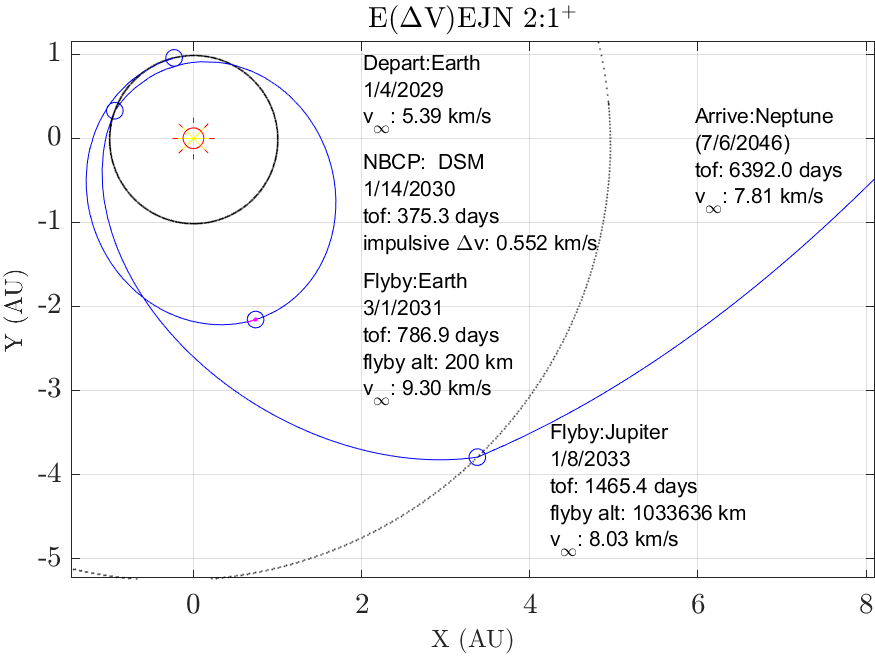
\includegraphics[width=1.0\textwidth]{./Figures/eejn21plus}
    \end{minipage}\hfill
		\begin{minipage}{0.50\textwidth}
				\centering
				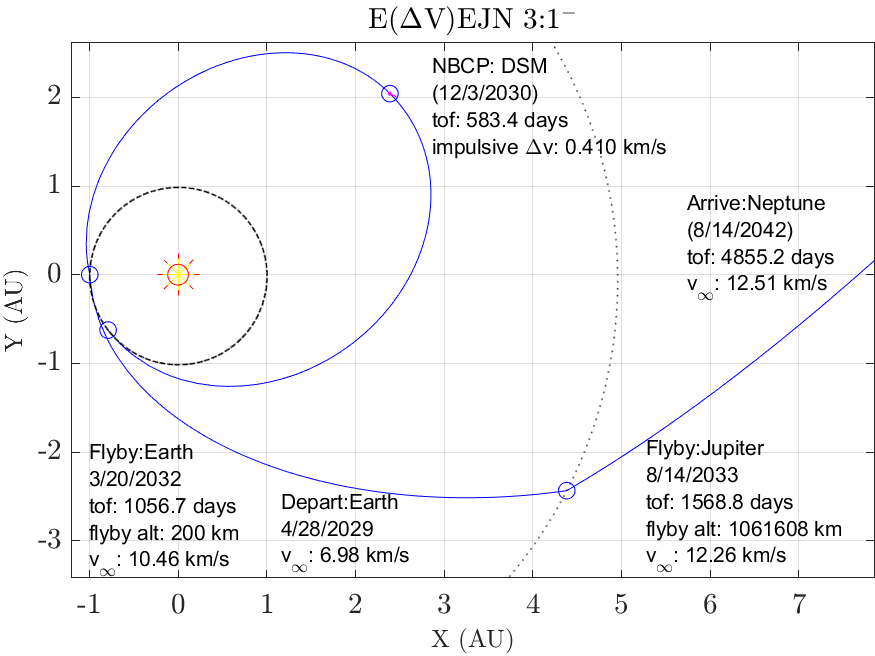
\includegraphics[width=1.0\textwidth]{./Figures/eejn31minus}
		\end{minipage}
		\caption{Optimized trajectory examples from the search. The left plot is an example of a 2:1$^{+}$ and the right is a 3:1$^{-}$. The 2:1$^{+}$ is able to reach Neptune with a much lower $V_\infty$ due to a slower relative velocity into Jupiter when compared to the 3:1$^{-}$ sequence.}
		\label{fig:maltotriton}
\end{figure}
%
%

Certain characteristics of the results were noticed when optimizing and comparing many cases from this tree search run. The deep space maneuver magnitude and direction general vary from the search results due to various factors. The optimization process takes into account the change in declination for the outgoing flyby so depending on the transfer an additional Z-component of velocity is expected. Another source of discrepancy is in the maneuver location. In the lookup table, the assumption is that the deep space maneuver is conducted at the aphelion of the leveraging orbit. However, the optimizer is able to shift the location of the maneuver within a reasonable time bound. In order to keep the look-up table two dimensional and to minimize the required $\Delta V$ at the aphelion, the minimizer was employed to reduce the normal component of velocity of the maneuver. This in turn limited solutions that may potentially have higher DSM $\Delta V$s for higher energy Earth gravity assists. It was also noticed that some trajectories from the search were exploiting the planar assumption resulting in lower launch velocities, DSM magnitudes, and flight times to Neptune. These limitations were only seen in the 2:1$^{-}$ set of solutions, which in theory have the lowest $\Delta V$ cost of any other trajectory type. However, with the solar system model used in MALTO, these sequences fall short due to energy limitations. When optimizing them, the largest discontinuous distance and velocity across all the segments of the trajectory was under 60,000 km and 0.2 $km/s$. The flight time and $V_\infty$ was also seen to reach the lower bound indicating a lower energy trajectory to Neptune (which is roughly 0.9 AU below the ecliptic plane in 2041).
































\clearpage
\noindent $\textbf{Notes}$
\\
\\\noindent Intro
		\\-We can remove the machine learning paragraph. We already mention the alg is heuristic free.
		\\-Should we mention rosetta if we don't prove it in the test cases?
		\\-Add a work scope (In this paper we are going to do ...)
\\
\\\noindent Theory
    \\-Theory $e_{out}$ needs to be defined in words (I assume its eccentricity from eq8)
		\\-Sentence starting with "Using the Newton..." is a fragment
		\\-"real life" under equation 9
		\\-"fuel usage" should be reworded?
		\\-comparing energy and vinf together (select 1 or the other)
		\\-DSM theory I use "we" but we dont really use we anywhere else in the theory
\\
\\\noindent Test Cases
		\\- maybe reword "no basis for its astrodynamics" (In order to test the algorithm's performance and ability to return useful sequence pairs...)
		\\-"Europa Clipper's" 3rd sentence in Performance Evaluation
		\\-push limits of powered flyby?
		\\-we can remove the "trident" name for Neptune trajectories bc they are not using EEVEE sequences.
		\\-The first case is a search to find a sequence similar to Europa Clipper's interplanetary trajectory (15F9-A22 EEVEEJ) utilizing multiple gravity assists of Earth and Venus to reach Jupiter[source].
		\\-maybe we should include a reminder of what d means?
		\\-"1.9 billion possible combinations possible..." reword
		\\-For Table 2 we should mention its dates for Europa Clipper and not Galileo in the caption.
		\\-After table 3, "An additional constrain"
		\\$<$got up to Figure 5$>$
		\\
	  \\-label for Table 8 in appendix to reference in text (I am using ref tab:tritontop25  right now in the text)


\phantom{p. 1}
\clearpage
\bibliographystyle{./AAS_publication}
\bibliography{./referencesDSMSsection}

\end{document}
